\section{Implementation and evaluation} \label{sec:eval}
We wish to have a practical technique for bounding floating-point round-off
error. To evaluate the practicality of our approach, we implement the type
inference algorithm detailed in this paper in Rust.
We evaluate our implementation on speed and precision of the analysis against
competiting tools on benchmarks in the FPBench benchmark suite \cite{fpbench}.
For our comparison, we use the precision specified in the corresponding FPBench
benchmark spec (e.g. \textsc{binary32}, \textsc{binary64}) and set the rounding
mode to round towards zero. 
% \footnote{The add-assoc benchmark is not from FPBench and is instead taken
% from our running example.}

\paragraph{Supported operations.}
Compared to Numerical Fuzz, our instantiation supports subtraction,
multiplication, and addition. We additionally support negative numbers. However,
we do not support division or taking square roots; we leave this as a potential
future direction in future work. 


\paragraph{Precision on absolute error.}
We compare the precision of our absolute error bounds against two alternative
approaches: FPTaylor \cite{fptaylor} and Gappa \cite{gappa}. In all of the
examples in Table~\ref{tab:bounds-abs}, we can see that NegFuzz's bounds are
tighter when \textbf{factor} is used.
We also observe that NegFuzz (with factor) obtains competitive bounds within an
order of magnitude with Gappa and FPTaylor, and occasionally produces tighter
bounds than Gappa.

\begin{footnotesize}
  \begin{table}[htbp]
\centering
\begin{tabular}{lllllllll}
\toprule
Benchmark & NegFuzz (no factor) & NegFuzz (with factor) & Gappa & FPTaylor &  &  &  &  \\
\midrule
sum & 2.665E-14 & 1.332E-14 & 6.661E-15 & 4.441E-15 &  &  &  &  \\
kepler0 & 9.534E-13 & 6.810E-13 & 1.982E-13 & 1.171E-13 &  &  &  &  \\
% shoelace-formula & 3.997E-09 & \textbf{1.998E-09} &  &  &  &  &  &  \\
himmilbeau & 4.746E-11 & 2.531E-12 & 2.000E-12 & 1.180E-12 &  &  &  &  \\
sineOrder3 & 9.385E-15 & 6.704E-15 & 2.069E-15 & 9.206E-16 &  &  &  &  \\
matrixDeterminant2 & 9.059E-11 & 2.665E-11 & 7.006E-12 & 3.126E-12 &  &  &  &  \\
rigidBody1 & 1.839E-12 & 1.532E-12 & 5.898E-13 & 4.263E-13 &  &  &  &  \\
delta4 & 1.144E-12 & 5.004E-13 & 1.768E-13 & 1.154E-13 &  &  &  &  \\
sqroot & 4.857E-15 & 1.332E-15 & 1.041E-15 & 9.714E-16 &  &  &  &  \\
rigidBody2 & 1.351E-09 & 6.757E-10 & 7.213E-11 & 4.543E-11 &  &  &  &  \\
matrixDeterminant & 9.059E-11 & 2.665E-11 & 7.006E-12 & 3.126E-12 &  &  &  &  \\
test01\_sum3 & 1.431E-05 & 7.153E-06 & 3.576E-06 & 2.384E-06 &  &  &  &  \\
kepler1 & 5.944E-12 & 2.843E-12 & 7.456E-13 & 3.918E-13 &  &  &  &  \\
% add-assoc* & 2.665E-12 & 1.776E-12 & 1.364E-12 & 9.095E-13 &  &  &  &  \\
\bottomrule
\end{tabular}
\caption{Comparison of the precision of NegFuzz (with and without
\textbf{factor}) against Gappa and FPTaylor. All bounds are absolute error
bounds.}
\label{tab:bounds-abs}
\end{table}
\end{footnotesize}

\paragraph{Precision on relative error.}
We now compare the precision of our relative error bounds. Note that
many of our example benchmark programs from FPBench contain subtraction or
negative numbers. This is a challenge for static numerical analysis tools to
determine if a program can output zero, which would make relative error
undefined.
In Table~\ref{tab:bounds-rel}, we compare the precision of our relative error
bounds against two alternative approaches.
In the sqroot benchmark, all tools manage to successfully bound away from zero
and obtain competitive error bounds.
% In the add-assoc and sqroot benchmark, all tools manage to bound away from zero.
% NegFuzz (with factor) produces the tightest error bound in add-assoc and
% produces competitive results in the sqroot benchmark. 

\begin{footnotesize}
\begin{table}[htbp]
\centering
\begin{tabular}{lllllllll}
\toprule
Benchmark & NegFuzz (no factor) & NegFuzz (with factor) & Gappa & FPTaylor &  &  &  &  \\
\midrule
sum &  &  &  & 1.011E-15 &  &  &  &  \\
kepler0 &  &  &  & 2.434E-15 &  &  &  &  \\
sqroot & 3.775E-15 & 1.332E-15 & 1.202E-15 & 8.883E-16 &  &  &  &  \\
test01\_sum3 &  &  &  & 5.427E-07 &  &  &  &  \\
kepler1 &  &  &  & 7.654E-15 &  &  &  &  \\
% add-assoc & 6.661E-16 & 4.441E-16 & 6.661E-16 & 2.22E-15 &  &  &  &  \\
\bottomrule
\end{tabular}
\caption{Comparison of the precision of NegFuzz (with and without
  \textbf{factor}) against Gappa and FPTaylor. All bounds are relative error
  bounds. Blank entries indicate where the tools had trouble bounding the result
  away from zero due to the presence of subtraction or negative numbers. On 8 of
the 14 benchmarks, all tools failed to bound away from zero and have been
omitted from the table for brevity.}
\label{tab:bounds-rel}
\end{table}
\end{footnotesize}

\paragraph{A posterori bounds.}
A posterori error bounds depend on the input of a program. To illustrate the
potential utility of a posterori absolute error bounds against the more standard
a priori error bounds given by Gappa and FPTaylor, we uniformly sample from the
input range of each benchmark and scatter-plot the corresponding bound. For the
benchmarks in Figure~\ref{fig:mixed-story} , we can see a mixed story: there are
program inputs under which NegFuzz will sometimes provide tighter absolute
error error bounds. For the other 11 benchmarks, the advantages of an a
posteriori error bound is less clear; Gappa and FPTaylor will produce tighter a
priori absolute error bounds.

\begin{figure}[h]
  \centering
  \begin{subfigure}{0.48\columnwidth}
    \centering
    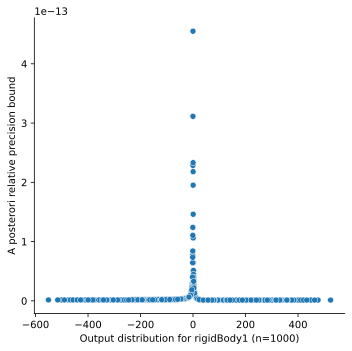
\includegraphics[width=\textwidth]{../plots/rigidBody1.pdf}
    % \caption{First diagram}
    \label{fig:sub1}
  \end{subfigure}
  \hfill
  \begin{subfigure}{0.48\columnwidth}
    \centering
    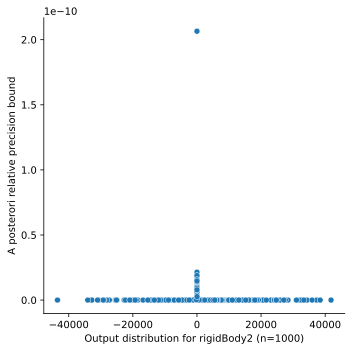
\includegraphics[width=\textwidth]{../plots/rigidBody2.pdf}
    % \caption{Second diagram}
    \label{fig:sub2}
  \end{subfigure}
  \hfill
  % \begin{subfigure}{0.32\columnwidth}
  %   \centering
  %   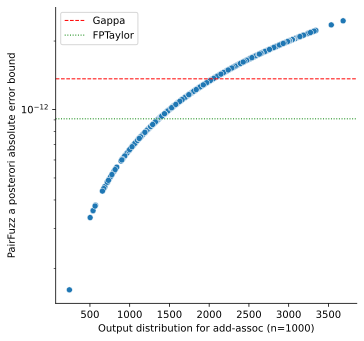
\includegraphics[width=\textwidth]{../plots/add-assoc.pdf}
  %   % \caption{Second diagram}
  %   \label{fig:sub2}
  % \end{subfigure}
  \caption{Plots of specific benchmarks where NegFuzz's posterori error bounds
    can sometimes be tighter than Gappa and FPTaylor. Each blue dot represents
    one input-output pair uniformly sampled from the input domain. The large
    dashed red lines represent the a priori absolute error bound given by Gappa
    and the smaller dashed green lines represent the a priori absolute error
    bound given by FPTaylor.}
  \label{fig:mixed-story}
\end{figure}

\paragraph{Performance.}
We now compare the performance of our NegFuzz implementation. Both FPTaylor and
Gappa take different time based on whether absolute or relative error is being
calculuated. As NegFuzz's error analysis relies only on the type information,
computing both the relative and absolute error bounds incurrs minimal overhead
compared to only computing one error bound. Accordingly, our implementation
reports both the relative and abslute error bounds simultaneously.

Several of the benchmarks take on the order of milliseconds for NegFuzz and
Gappa to compute. To minimize system noise due to disk reading and caches, we
measure each benchmark by running the benchmark 5 times to warmup the disk
caches and take the median wall-clock time of 50 benchmark runs. All
measurements were taken on a Framework Laptop 13 with a 12th Generation Intel
i7-1280P CPU and 64 GB of RAM on a Debian operating system running in a Xen
hypervisor. 

As shown in Table~\ref{tab:perf}, we consistently outperform Gappa and FPTaylor,
often by an order of magnitude or more. Moreover, programs using the
\textbf{factor} primitive are faster than the same program written without
factor in all but one of our benchmarks.

\begin{footnotesize}
\begin{table}[htbp]
\centering
\begin{tabular}{llllllllll}
\toprule
Benchmark & Gappa (abs.) & Gappa (rel.) & NegFuzz (no factor) & NegFuzz (with factor) & FPTaylor (rel.) & FPTaylor (abs.) \\
\midrule
sum & 0.02253 & FAIL & 0.005026 & \textbf{0.00447} & 0.781 & 0.3981 \\
kepler0 & 0.04553 & FAIL & 0.007683 & \textbf{0.008623} & 2.28 & 14.85 \\
himmilbeau & 0.03927 & FAIL & 0.003182 & \textbf{0.003287} & FAIL & 0.03008 \\
sineOrder3 & 0.01593 & FAIL & 0.00167 & \textbf{0.002106} & FAIL & 0.02709 \\
matrixDeterminant2 & 0.1606 & FAIL & 0.007249 & \textbf{0.005932} & FAIL & 13.73 \\
rigidBody1 & 0.02717 & FAIL & 0.004609 & \textbf{0.004177} & FAIL & 0.2007 \\
delta4 & 0.09792 & FAIL & 0.01109 & \textbf{0.008473} & FAIL & 0.8243 \\
sqroot & 0.07071 & 0.03826 & 0.007927 & \textbf{0.005462} & 0.02272 & 0.02017 \\
rigidBody2 & 0.02908 & FAIL & 0.008406 & \textbf{0.005789} & FAIL & 0.2029 \\
matrixDeterminant & 0.08021 & FAIL & 0.01281 & \textbf{0.005085} & FAIL & 13.9 \\
test01\_sum3 & 0.03723 & FAIL & 0.005074 & \textbf{0.004452} & 1.074 & 0.4695 \\
kepler1 & 0.1617 & FAIL & \textbf{0.01291} & 0.0153 & 0.2746 & 14.1 \\
% add-assoc* & 0.01283 & 0.01406 & 0.002355 & \textbf{0.002266} & 0.2179 & 6.139 \\
\bottomrule
\end{tabular}
\caption{End to end timings of each tool run on each benchmark in seconds. Each
  tool is broken out by the type of error analysis that was performed. As our
  approach only relies on type-checking, our implementation does not take extra
  time to compute both absolute and relative error; we report both error bounds
  simultaneously. Results reported are the median wall-clock time out of 50
  benchmark runs.}
\label{tab:perf}
\end{table}
\end{footnotesize}

\subsection{Evaluation takeaways}
From our evaluation tables and figures, we make four claims:

\paragraph{Our type-based approach is faster than competing approaches.} On our
the benchmarks taken from FPBench that our tool supports, our approach is
signficantly faster than competing approaches, often outperforming by an order
of magnitude. In fact, on the benchmarks we evaluated against, our
implementation was so fast that we found that our parsing and disk reading times
often dominated the total execution time.

\paragraph{Our type-based approach yields useful a priori bounds that are
competitive with other competing approaches.} Our work is the first type-based
approach that is able to reason about forwards round-off error in the presence
of subtraction and negative numbers. Both the absolute error bounds that we
achieve are often comparable to state-of-the-art tools such as Gappa and
FPTaylor. Futher, when tools are able to bound away from zero and provide a
relative error bound, our approach occasionally able to do the same.

\paragraph{A posteriori error bounds can be useful in obtaining tighter
round-off error analyses} We observe our approach on concrete program executions
often produces competitive error bounds. In some circumstances, our type-based
approach can produce a posteriori error bounds that are tighter than Gappa and
FPTaylor. We also observe that our a posteriori error bounds are cheap and
practical to compute given a concrete program output.

\paragraph{The \textbf{factor} primitive results in tighter error bounds and
faster type-checking.} We observe that using the \textbf{factor} in our programs
always results in tighter error bounds for the same underlying computation.
Often times our bounds are signifiantly smaller and occasionally they are an
order of magnitude smaller. We also observe that \textbf{factor} often resulted
in faster type-checking, outperforming the equivalent program without
\textbf{factor} in all but one of the benchmark programs.
